%%%%%%%%%%%%%%%%%%%%%%%%%%%%%%%%%%%%%%%%%
% Homework Assignment Article
% LaTeX Template
% Version 1.3.1 (ECL) (08/08/17)
%
% This template has been downloaded from:
% Overleaf
%
% Original author:
% Victor Zimmermann (zimmermann@cl.uni-heidelberg.de)
%
% License:
% CC BY-SA 4.0 (https://creativecommons.org/licenses/by-sa/4.0/)
%
%%%%%%%%%%%%%%%%%%%%%%%%%%%%%%%%%%%%%%%%%

%----------------------------------------------------------------------------------------

\documentclass[a4paper]{article} % Uses article class in A4 format

%----------------------------------------------------------------------------------------
%	FORMATTING
%----------------------------------------------------------------------------------------

\addtolength{\hoffset}{-2.25cm}
\addtolength{\textwidth}{4.5cm}
\addtolength{\voffset}{-3.25cm}
\addtolength{\textheight}{5cm}
\setlength{\parskip}{0pt}
\setlength{\parindent}{0in}

%----------------------------------------------------------------------------------------
%	PACKAGES AND OTHER DOCUMENT CONFIGURATIONS
%----------------------------------------------------------------------------------------

\usepackage{blindtext} % Package to generate dummy text
% \usepackage[style=numeric,sorting=none]{biblatex}
\usepackage{charter} % Use the Charter font
\usepackage[utf8]{inputenc} % Use UTF-8 encoding
\usepackage{microtype} % Slightly tweak font spacing for aesthetics

\usepackage[english]{babel} % Language hyphenation and typographical rules

\usepackage{amsthm, amsmath, amssymb} % Mathematical typesetting
\usepackage{float} % Improved interface for floating objects
\usepackage[final, colorlinks = true, 
            linkcolor = black, 
            citecolor = black]{hyperref} % For hyperlinks in the PDF
\usepackage{graphicx, multicol} % Enhanced support for graphics
\usepackage{xcolor} % Driver-independent color extensions
\usepackage{marvosym, wasysym} % More symbols
\usepackage{rotating} % Rotation tools
\usepackage{censor} % Facilities for controlling restricted text
\usepackage{listings, style/lstlisting} % Environment for non-formatted code, !uses style file!
\usepackage{color}

\definecolor{dkgreen}{rgb}{0,0.6,0}
\definecolor{gray}{rgb}{0.5,0.5,0.5}
\definecolor{mauve}{rgb}{0.58,0,0.82}
\lstset{frame=tb,
  language=Java,
  aboveskip=3mm,
  belowskip=3mm,
  showstringspaces=false,
  columns=flexible,
  basicstyle={\small\ttfamily},
  numbers=none,
  numberstyle=\tiny\color{gray},
  keywordstyle=\color{blue},
  commentstyle=\color{dkgreen},
  stringstyle=\color{mauve},
  breaklines=true,
  breakatwhitespace=true,
  tabsize=3
}
\usepackage{pseudocode} % Environment for specifying algorithms in a natural way
\usepackage{style/avm} % Environment for f-structures, !uses style file!
\usepackage{booktabs} % Enhances quality of tables

\usepackage{tikz-qtree} % Easy tree drawing tool
\tikzset{every tree node/.style={align=center,anchor=north},
         level distance=2cm} % Configuration for q-trees
\usepackage{style/btree} % Configuration for b-trees and b+-trees, !uses style file!

% \usepackage[backend=biber,style=numeric,
            % sorting=nyt]{biblatex} % Complete reimplementation of bibliographic facilities
% \addbibresource{ecl.bib}
\usepackage{csquotes} % Context sensitive quotation facilities

\usepackage[yyyymmdd]{datetime} % Uses YEAR-MONTH-DAY format for dates
\renewcommand{\dateseparator}{-} % Sets dateseparator to '-'

\usepackage{fancyhdr} % Headers and footers
\pagestyle{fancy} % All pages have headers and footers
\fancyhead{}\renewcommand{\headrulewidth}{0pt} % Blank out the default header
\fancyfoot[L]{School of Computing, Macquarie University} % Custom footer text
\fancyfoot[C]{} % Custom footer text
\fancyfoot[R]{\thepage} % Custom footer text

\usepackage{comment}
\newcommand{\note}[1]{\marginpar{\scriptsize \textcolor{red}{#1}}} % Enables comments in red on margin

\hypersetup{
    colorlinks=true,
    linkcolor=blue,
    filecolor=magenta,      
    urlcolor=cyan,
    pdftitle={COMP3100 Stage 1 Report},
    pdfpagemode=FullScreen,
    }

%----------------------------------------------------------------------------------------

\begin{document}

%----------------------------------------------------------------------------------------
%	TITLE SECTION
%----------------------------------------------------------------------------------------

\title{COMP3100 project report} % Article title
\fancyhead[C]{}
\hrule \medskip % Upper rule
\begin{minipage}{1\textwidth} % Center of title section
\centering 
\large % Title text size
Project report: Stage 1\\ % Assignment title and number
COMP3100 Distributed Systems, S2, 2022\\
\normalsize % Subtitle text size
SID: 45456070, Name: Beau Williams
%%%%\\ % Assignment subtitle
\end{minipage}
\medskip\hrule % Lower rule
\bigskip

%----------------------------------------------------------------------------------------
%	ARTICLE CONTENTS
%----------------------------------------------------------------------------------------

\section*{1. Introduction}
For this COMP3100 assignment we are tasked with building a client side interface for the Distributed Systems Server Simulator (DSSIM)\cite{dssim} that implements a job scheduler using the Largest Robin Round (LRR) algorithm and later on more algorithms and features. This report shall cover stage 1 of this assignment, which involves the implementation of the LRR Scheduler, as well as interfacing with the DSSIM to perform a hanshake process and then schedule the jobs until there are no more left, at which point the client terminates the session with DSSIM.
\newline

The purpose of the report coupled with the design and implementation of the client side code is intended to introduce students to various aspects relating to the design and implementation of a distributed system, along with consideration of algorithms used to orchestrate these systems efficiently.
\newline

In this report, there shall include a system overview of DSSIM, a discussion on the design philosophy that drove the implementation of the client side architecture, as well as a detailed overview of that implementation. Also discussed will be other notable matters relating to the DSSIM, client interface and distributed systems architecture.

\section*{2. DSSIM System Overview}

At a high level, the job scheduling system that we are creating adopts a client-server architecture. It is made of to main components, the server being the DSSIM binary written in imperative C[1] and the client being written in object-oriented java. This combination allows the server to operate at a much greater efficiency, while allowing the client structure to be more composable.

The DSSIM is designed to operate servers and dispatch jobs to them, as opposed to the clients role to orchestrate the dispatching of jobs to the servers. The DSSIM is concerned with the generation of events, as well as the state and configuration of servers at the DSSIM's disposal. Events in the DSSIM are messages, such as "HELO" and "QUIT", each of these messages corresponds to a particular event in the DSSIM, where it can either be the client sending or receiving events to the DSSIM.
\newline

Between the client and the server is an initial handshake process as defined by the Handshake Protocol. Breifly, this involves the client connecting to the server through a Transmission Control Protocol (TCP) socket connection, sending "HELO", receiving "OK", sending "ATUH user", and receiving a final "OK" to confirm the handshake has completed. Upon completion of this handshake, the client will have access to read through the jobs that are defined in a markup (xml) file optionally. 
\newline
At this stage the client will state they are ready to begin orchestrating jobs to servers be sending a "REDY" message, at which point the server will respond with "JOBN [submitTime] [jobID] [estRuntime] [core] [memory] [disk]". The client will then retrieve the capable servers using  “GETS Capable [job information]”. The client will then receive a message "DATA [numServers] [numJobs]" followed by a list of capable servers, responding "OK" to the server to acknowledge receipt of the message, signalling the server to send the next message. \newline
Finally, the client will begin to schedule the jobs to the server at its own discretion according to the orchestration algorithm such as LRR, sending each job as a message "SCHD [jobID] [serverType]" to the DSSIM. Once the jobs have been dispatched a final "NONE" message will be received, at which point the client can choose to respond with "OK" and "QUIT" to terminate the session.
\newline

Given the decoupled nature of the client and server, and the simplicity of message passing, DSSIM and client are designed to work across many communication methods such as Remote Procedure Calls (RPC), through a TCP socket interface. The client and server can be located on any machine. The caveat being that only messages can be passed between the client and the server, which means rich two-way communication is not possible, however this is not at all necessary.
\newline
\subsection*{2.1. System Diagram}
The DSSIM System is shown below at a high level by figure \ref{DSSIM}
\begin{figure}[H]
    \centering
    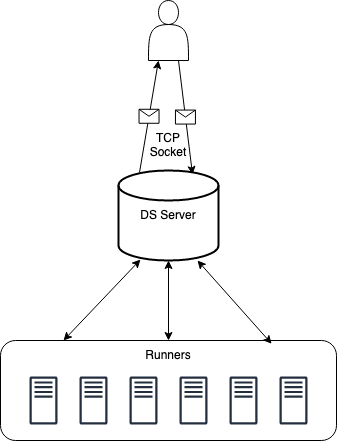
\includegraphics[scale=0.6]{images/DSServer.png}
    \caption{DSSIM System Design}
    \label{DSSIM}
\end{figure}


\section*{3. Client Design}
\subsection*{3.1. Design Philosophy}
The philosophy behind the client design is to separate concerns in such a manner that the development of the client implementation can occur in a distributed fashion, while also paying attention to the workings of the short term memory (limited in how many things we can keep track of at any one time). I chose to separate the concerns into four parts at the high level, client "controller", server "interface", data "objects", scheduler "algorithms".
\newline
The key reason to firstly start by implementing an interface coupled with a controller was to decouple the implementation logic relating to client to server messaging service, from the implementation logic that describes the controller and its parts.
\newline
Following this, I have abstracted the data objects, this allows developers working on the client to have more contextual information presentation of data returned from the DSSIM using the type system built into java. Additionally, this allows effective consumption and present data in a structured fashion throughout the programs lifecycle.
\newline
Lastly, we find the Scheduler class algorithm objects, these are controlled by the client, consume data objects, and interface with the DSSIM. For our client this means that implementing a controller is as easy as instantiating the DSServerInterface class as well as a chosen Scheduler algorithm, in order to perform the process of orchestrating jobs to the DSSIM.
\subsection*{3.2. System Diagram}
The client design is shown below at a high level by figure \ref{CLIENT}
\begin{figure}[H]
    \centering
    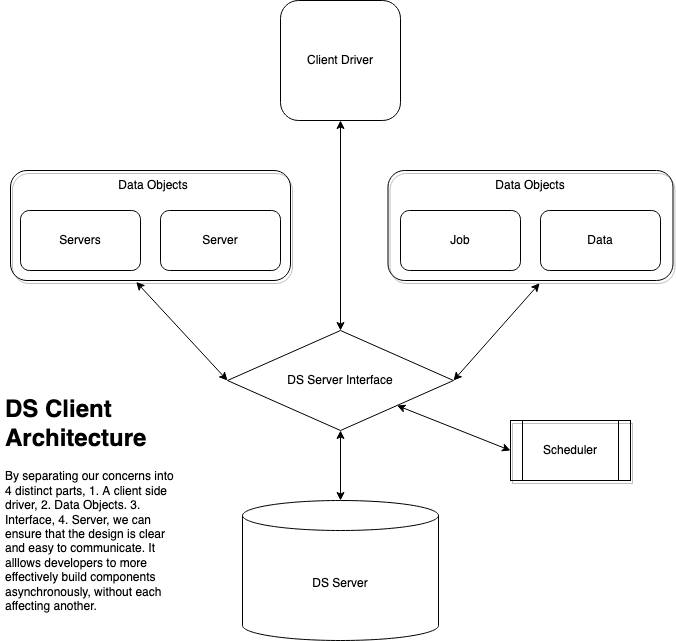
\includegraphics[scale=0.7]{images/DSClient.png}
    \caption{DSSIM Client Design}
    \label{CLIENT}
\end{figure}

\section*{4. Implementation}
The implementation of the client interface for DSSIM follows an object oriented style, with a focus on cleanliness, testable code, as well as extensibility and composobility. Below I will detail the core comnponents of the client side architecture, and how they are implemented.

\subsection*{4.1. Tooling}
This project was built with the help of a modal text editor neovim\cite{neovim}, coupled with the the Language Server Protocol (LSP)\cite{lsp} providing contextual feedback on errors, code suggestions and more language related feedback. Our client and server is hosted on a VM using multipass, a Ubuntu container orchestrator built by Canonical. Lastly we use a task runner called just combined with shell scripts to automate testing, deployment and operation of the DSSIM.

\subsection*{4.2. Libraries}
\begin{itemize}
    \item java.io*
    \item java.util.ArrayList
    \item java.util.List
    \item java.util.Iterator;
\end{itemize}



\subsection*{4.3. DSSIM Interface}

The DSSIM Interface provides helper methods that allow for the Client, and Objects and Scheduler to communicate back and forth with the dsserver.

Here we also codify the specifics relating to the implementation of the dsserver interface. Such as available commands. Methods, types and more.
\begin{figure}[ht!]
\begin{lstlisting}
  public DSInterface(String host, int port) {
    this.host = host;
    this.port = port;
    this.connected = false;
  }

  private String[] split(String s) { return s.split(" "); }

  public void connect() throws IOException {
    socket = new Socket(host, port);
    in = new BufferedReader(new InputStreamReader(socket.getInputStream()));
    out = new PrintWriter(socket.getOutputStream(), true);
    connected = true;
  }

  public void disconnect() throws IOException {
    if (connected) {
      socket.close();
      connected = false;
    }
  }

  public void send(String msg) throws IOException { out.println(msg); }

  public String receive() throws IOException {
    try {
      return in.readLine();
    } catch (IOException e) {
      System.out.println("");
      return null;
    }
  }
\end{lstlisting}
\caption{The DSInterface Object}
\end{figure}




\subsection*{4.4. DSSIM Client}

Our DSSim client is deceptively simple. We can implement a more user friendly controller interface now, but as shown, in order to complete the task of orchestrating and scheduling the jobs to DSSIM, most of the implementation is abstracted. All that is required becomes a 4 step process that is logical and easy to follow. 1. connect 2. authenticate 3. schedule jobs 4. disconnect.


\begin{figure}[ht!]
\begin{lstlisting}
      DSInterface dsserver = new DSInterface(host, port);
      Scheduler scheduler = new Scheduler();
      dsserver.connect();
      dsserver.authenticateUser();
      scheduler.lrrScheduler(dsserver);
      dsserver.send(dsserver.QUIT);
      dsserver.disconnect();
\end{lstlisting}
\caption{The DSClient Controller}
\end{figure}

\subsection*{4.5. Data Objects}

We have defined objects such as Server, Servers, Job and Data to encapsulate the logic related to these objects as well as define an interface, set the types and methods available to each of these objects. By using objects, we can more effectively model the data within our application. Allowing for the client interface to become more composable.

\begin{figure}[ht!]
\begin{lstlisting}
  public Server(String server){
    String[] serverInfo = server.split(" ");
    this.type = serverInfo[0];
    this.id = Integer.parseInt(serverInfo[1]);
    this.state = serverInfo[2];
    this.hourlyRate = Integer.parseInt(serverInfo[3]);
    this.core = Integer.parseInt(serverInfo[4]);
    this.memory = Integer.parseInt(serverInfo[5]);
    this.disk = Integer.parseInt(serverInfo[6]);
  }

\end{lstlisting}
\caption{The server data object}
\end{figure}

\subsection*{4.6. Scheduler}
\subsubsection*{4.6.1. Last Round Robin}
The implementation of the Last Round Robin (LRR) uses a simple while loop combined with a conditional break, which is triggered when the server sends "NONE". Specifically, the jobs in the LRR algorithm are scheduled as such that the jobs are dispatched to the servers with the highest core counts. However, in the case of a tie between two or more servers of which have an equally high core count, the first discovered server will be chosen. The type of that server will be stored in a variable. Jobs will only be dispatched to the server of that type. The DS Client will filter the list of capable servers by the server type using the DS Server interface. The LRR algorithm will then send jobs to the list of servers, iterating by one each time. Eventually, as the server index in the list exceeds the number of servers in the list, the LRR algorithm will repeat the "round robin" starting again with the first index, and will continue to iterate through the server list, dispatching jobs to each of the largest servers by type, until there are no more jobs left. Once the LRR algorithm receives status code message back from DSSIM "NONE" it will cease sending jobs and the LRR algorithm will exit.

\section*{Conclusion}
This report has demonstrated the purpose behind building a distributed system such as the DSSIM, and how it might be utilised and implemented. We have discussed my choices for design philosophy relating to the client side interface, and why this approach is justified. We have also shown how various technologies, programming paradigms and computers can communicate with each other to produce effective collective action. We can see that the design of a client application will often differ from the design of a server application. Where the client side is focussed on composability, ease of access and extensibility, whereas the server is designed to be robust, fault tolerant, efficient. We have also discussed why such a design might be favourable, and how decoupling and separating concerns in a process lifecycle can provide numerous benefits such as allowing for discrete and distributed development of the parts that make up the systems whole.


\subsection*{Source Code Repository}
\begin{itemize}
    \item \hyperlink{https://github.com/beauwilliams/Comp3100}{Github repository}
\end{itemize}

%----------------------------------------------------------------------------------------
%	REFERENCE LIST
%----------------------------------------------------------------------------------------
\bibliographystyle{ieeetr}
\bibliography{comp3100project}
% \printbibliography

%----------------------------------------------------------------------------------------

\end{document}
